\cotefile{15}

\scanpage{180}

\begin{center}
Calculs de cohomol. absolue\\
du motif de Tate\\
$\unsure{\mathbf Z|N}(n)$.
\end{center}

\margin{179}

\scanpage{183}
Soit $\mathcal M$ une catégorie de motifs géométriques, \inserted{de type fini,} sur le préschéma $S$ de type fini sur $\mathbf Z$. Pour simplifier, supposons que les degrés de $\mathcal M$ soient pairs (sinon, il sera possible, pour \deleted{la plupart des} \inserted{certaines} questions de distribution des Frobenius, de remplacer $\mathcal M$ par $\mathcal M^{\mathrm{pair}}$). Tout choix d'un pt fermé $s\in S$ permet donc, de définir des (une collection de) ``$\mathbf R$-points Motiviques'' \deleted{\unsure{point de vue}''} \inserted{de $\mathcal M$}.

Pour fixer les idées, choisissons un pt $\mathbf R$-motivique de $\mathcal M$, d'où un gpe physique $G_{\mathbf R}$ sur $\mathbf R$.

Il y a lieu de \deleted{dupliquer} \inserted{démultiplier} les point \inserted{fermés $s$} de $S$, en formant les couples $s'=(s,\unsure{i|i'})$, où $s\in S^0$, et
\margin{l'exposant $0$ désigne des pts \uline{fermés}}
$i_{\deleted{\unsure{s|x}}}\colon G_{m\,\mathbf C}-G(s)_{\mathbf C}$ est de type \deleted{\unsure{divisé|désigné}} préférentiel --- $G(s)$ désigne le gpe de Galois motivique associé à $\mathcal M_s$.

\deleted{Alors} Soit $S'$ l'ens de ces couples. A tout $s'\in S'$ est associé un $\mathbf R$-point motivique de $\mathcal M$, \deleted{d'où un} déterminé à isom près, d'où un $\zeta(s')\in H^1(\mathbf R,\deleted{F}G_{\mathbf R}^{\mathrm{or}})$, où $G^{\mathrm{or}}$ est le noyau de $G_{\mathbf R}^0\xrightarrow{\varepsilon}G_m$. De plus, si $G_{\mathbf R}^{\zeta(s')}$ est ``le'' gpe déduit de $G_{\mathbf R}$ par torsion par $\zeta(s')$, on obtient un hom
\[
u(s')\colon G(s')_{\deleted{\unsure{R|k}}\mathbf R}=G(s)_{\mathbf R}\longrightarrow G_{\mathbf R}^{\zeta(s')}
\]
compatible avec $\varepsilon_{\mathbf R},J_{\mathbf R}$, et déterminé en fait mod \deleted{\unsure{automorphisme|automorphismes}} \inserted{conjugaison} \deleted{\unsure{intérieur|intérieurs}} par un élément de $G_{\mathbf R}^{\mathrm{or}}(\mathbf R)$.
\margin{182}

\scanpage{184}
\mspage{73}

a homomorphism of restriction of a function on $\mathcal E_{\varphi}$. We obtain from (16):
\[
0\to O_V(-\mathcal E_{\varphi})[nE]\to O_V[nE]\xrightarrow{r'}O_{\mathcal E_{\varphi}}[nE]_{\mathcal E_{\varphi}}\to 0\qquad(17)
\]
here $r'$ is such: if $P\notin\mathcal E_{\varphi}$, then it is a zero homomorphism; if $P\in\mathcal E_{\varphi}$ and $\{\alpha^{(i)}\}\in O_V[nE](P)$, then $r'\{\alpha^{(i)}\}=\{r\alpha^{(i)}\}$. To the sequence (17) corresponds such exact sequence:
\[
\begin{aligned}
&H^0(V,O_V[nE])\xrightarrow{r^*} H^0(\mathcal E_{\varphi},O_{\mathcal E_{\varphi}}[nE]_{\mathcal E_{\varphi}})\to H^1(V,O_V(-\mathcal E_{\varphi})[nE])\to\\
&\to H^1(V,O_V[nE])\to H^1(\mathcal E_{\varphi},O_{\mathcal E_{\varphi}}[nE]_{\mathcal E_{\varphi}})
\end{aligned}
\qquad(18)
\]

Let $n(\mathcal E_{\varphi})$ be such that, at $n\geq n(\mathcal E_{\varphi})$ for $\mathcal E_{\varphi}$ and $[nE]_{\mathcal E_{\varphi}}$ satisfy the requirements $1')$ and $2')$ (See p. 202). The existence of such $n(\mathcal E_{\varphi})$ follows from the condition of non-degeneracy of $[E]_{\mathcal E_{\varphi}}$ over $\mathcal E_{\varphi}$. Put
\[
n_{\mathcal E}=\max(n'',\,n(\mathcal E_{\varphi})).
\]

Then, at $n\geq n_{\mathcal E}$, from (15), (18) and from the fact that, at $n\geq n(\mathcal E_{\varphi})$
\margin{183}

\scanpage{185}
De plus, on a une structure polarisée\inserted{ $\pi$} sur $G_{\mathbf R}^{\circ}$, qu'on peut \deleted{\unsure{défi|définir}} supposer définie par un hom \deleted{$\unsure{\mu_2\to G}$} $i:\mu_{2\,\mathbf C}\longrightarrow G_{\mathbf C}^{\circ}$ (comme on voit en envoyant un tore \inserted{provenant d'un $s$} dedans). D'autre part, $G(s')_{\mathbf C}$ est muni de $i(s'):G_{m\,\mathbf C}\to G(s')_{\mathbf C}$, et \unsure{on|qu'on} obtient par conséquent
\[
\unsure{v_{\zeta}|v_1}(s')=u(s')_{\mathbf C}\circ\bigl(i(s')\mid\mu_2\bigr):\mu_{2\,\mathbf C}\longrightarrow G_{\mathbf C}^{\zeta(s')}
\]
\deleted{D'autre part,} Ceci posé, il faut que $\pi^{\zeta(s')}$ (polarisation de $G_{\mathbf R}^{\zeta(s')}$ déduite de $\pi$ sur $G$ par transport) soit celle définie par les $\mu_{2\,\mathbf C}$. Par conséquent, pour $s'$ variable de façon que $\zeta(s')$ reste constant, les polarisations \inserted{de $G_{\mathbf R}^{\zeta(s')}$} associées aux différents $v(s')$ doivent être identiques -- ce qui donne une condition non tautologique sur la distribution des \deleted{\unsure{$v$}} $u(s')$. [Noter cependant que l'ens des \deleted{classes de} polarisations d'un gpe réel \inserted{$H$}, défini en termes d'hom $\mu_{2\,\mathbf C}\to H_{\mathbf C}$, \margin{? à vérifier} est \uline{fini}, [si $G$ est commutatif en tous cas !], donc la restriction n'est pas tellement draconienne.

Enfin, conformément aux conjectures de Tate magnifiées, la connaissance des $u(s')$ permet de retrouver la structure d'effectivité dans la catégorie
\margin{184}

\scanpage{187}
des $G_{\mathbf R}$-modules de dim finie sur $\mathbf R$. Le cône qui exprime cette effectivité est \uline{engendré} par les \deleted{$u(s')$} rayons définis par les $v(s')$. C'est un fait qui exprime \inserted{sous forme ``analytique''} le fait que les frobénius $f(s')\in G_{\mathbf R}^{\zeta(s')}(\mathbf R)$ ont la vertu que leurs valeurs propres, dans tte représentation de $G_{\mathbf R}^{\zeta(s')}\deleted{(\mathbf R)}$ -- et en fait $=$ de $G_{\deleted{\mathbf R}\mathbf C}^{\zeta(s')}$ -- sont des \uline{entiers} algébriques, ce qui est une condition arithmétique assez draconienne !
\margin{186}

\scanpage{189}

\begin{center}
\uline{Théorie de Galois des Motifs}

\uline{Généralités}
\end{center}

\margin{188}

\scanpage{190}

\begin{flushright}
Foncteurs fibres motiviques\\
et gp fondamental\\
motivique
\end{flushright}

\margin{189}

\scanpage{191}
$X$ préschéma connexe, \deleted{\unsure{(réduite, ce qui ne restreint p|réduit, ce qui ne restreint p}}

$1^\circ)$ $X_{\mathrm{réd}}$ de car $p>0$. Alors dans le pro-torseur fondamental $(T_\alpha)$, il n'y a pas en général de sections pour les $T_\alpha$. \deleted{On} On dispose uniquement, \deleted{de façon canonique}

(i) des $\xi_{\ell}^{(\alpha)}\in T_\alpha(\mathbf Z_{\ell})$, $l\ne p$, provenant sans doute de $\xi_{\ell}\in T_\alpha(\widetilde{\mathbf Z}_{\ell\mathbf Z})$
\margin{Coh. $l$-adique}
\margin{hensélisé}

\diagram{\begin{tikzcd}[ampersand replacement=\&,column sep=0pt,row sep=3.3em]
\text{(ii) d'un }\xi_p^{(\alpha)}\in T_\alpha( \& \mathbb{W}_p(k)\arrow[dr,swap,"{\text{``DeRham-Hodge''}}"] \& )\quad\text{si } \deleted{X\ \text{de t.f. sur}}\inserted{\text{$k$ est un}}\ \inserted{\text{corps parfait sur $X$}}\,\deleted{\text{le corps parfait }k} \\
\text{(iii) }\bigl[\,?\quad\text{\uline{réduit}}\ \xi_p^{(\alpha)\,0}\in T_\alpha( \& \deleted{\mathbb{W}}\ \& k\,)\ \bigr]
\end{tikzcd}}
\margin{\figure{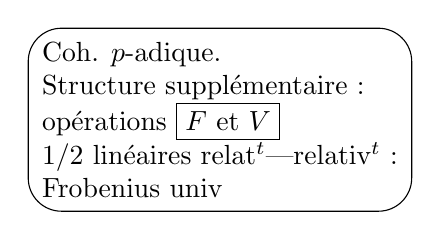
\begin{tikzpicture}
\node[draw,rounded corners=12pt,align=left,inner sep=5pt] {Coh. $p$-adique.\\Structure supplémentaire :\\opérations \fbox{\uuline{$F$} et \uuline{$V$}}\\$1/2$ \uuline{linéaires} \uuline{\unsure{relat$^t$|relativ$^t$}} :\\Frobenius univ};
\end{tikzpicture}}}
\margin{Coh. Hodge-de Rham Mais ici, il faut \deleted{sans doute} donc aller dans la catégorie $\overline{\unsure{M|\mathcal{M}}}$ dérivée. Tenir compte aussi de la structure \uline{filtrée} en Hodge-De Rham}

[$\xi_p$ provenant sans doute d'un $\xi_p\in T_p(\overset{\sim\!\sim}{\mathbf Z}_{p\mathbf Z})$]\margin{hensélisé strict.}

\margin{\unsure{N.B.}}
Si $X=\operatorname{Spec}\mathbf F_q$, il y a en général des \deleted{\unsure{pts}} obstructions non triviales dans des $H^2(\mathbf Q,G)$ \ldots

\deleted{On} On utilise des ``foncteurs fibres'' qui induisent sur les motifs effectifs de poids $0$ le foncteur canonique. Alors les \unsure{objets|d pts} de $T_\alpha(\mathbf Z_\ell)$ sont sans doute uniques \inserted{à isom près}, (th. de Lang), de $=$ ceux de $T_\alpha(\deleted{\unsure{\mathbf Z}}\mathbb{W}_p(k))$ si $k$ fini (id), \inserted{plus gén.} pour un $k$ parfait de dim ch $1$ (?). En général, il faut s'attendre que $T_\alpha(k)$ \deleted{soit un} ait plus d'un élément à isom près, mais il est possible que $T_{\deleted{\unsure{\alpha|\infty}}}(k)=\varprojlim T_\alpha(k)$ n'a qu'un élément à isom près, celui donné par la théorie de DeRham-Hodge.
\margin{relation avec les problèmes galoisiens ?? Il doit être \uline{équivalent}, cf \uline{Manin}}
\margin{190}

\scanpage{192}
ALGÈBRES de LIE SEMI-SIMPLES \mspage{(9)}\hfill Tribu n\textsuperscript{o} 59

Pas de noms propres à la p. 55 ; Chevalley et Harish on parlera longuement de dans la note historique. Dans la prop. 7 appeler les gens donnés $X'$ et $Y'$. Au lieu du ``tout de suite'', (l.2, p. 56), dire pourquoi, (ça se propage à partir des racines simples).

Utiliser le lemme sur les applications $R\longrightarrow\text{groupe}$ au milieu de la p. 56. Ensuite poser $X_\alpha=u_\alpha^{-1}X'_\alpha$, (alors $t_\alpha=1$). Pas de nom à la p. 57.

\uline{Exer6} - Dans l'exer. 3 donner le système des $h$, $x$, $y$ de Weyl, qui fournit des formules sans dénominateurs. Donner la démonstration Van der Waerden, (cf. Jacobson, bas p. 123 et p. 124).

\S\,4 - \uuline{Théorèmes d'existence}, (nouveau titre).

Dans ce \S\ on fait deux constructions distinctes, qui amènent presque aux mêmes résultats. On en laissera tomber une, d'où disparition des th. 3 et 4. Ceci amène au plan suivant :

1) Construction de $\underline{a}=\underline{x}+\underline{h}+\underline{y}$ ;

2) Définition des gros modules $E(\lambda)$ ; liberté de $\underline{x}$ et $\underline{y}$ ;

3) Construction de $\underline{g}$ comme quotient de $\underline{a}$ par les $\unsure{\Theta|\theta}_{ij}$ ; alors $\underline{g}=\underline{h}+\sum_{\lambda}\underline{g}^{\lambda}$, est de dim. finie, et est semi-simple ;

4) Définition des $W(\lambda)$ ; sont des $g$-modules ;

5) $W(\lambda)$ est de dim. finie si $\lambda$ est un pouah dominant ; conséquences pour $\underline{g}$.

Dans 3) la semi-simplicité de $\underline{g}$ se démontre ainsi : on a $[\underline{g}^{\alpha},\underline{g}^{-\alpha}]=\underline{h}^{\alpha}$, (vrai pour $\alpha$ simple, et $W$ opère) ; alors tout idéal commutatif $\underline{b}$ est nul, (car $\underline{b}\cap\underline{s}_\alpha=0$ pour toute sous-algèbre $\underline{s}_\alpha$ de dim. 3). A partir de là tous les cor. concernant $\underline{g}$ se démontrent facilement.
\margin{191}

\scanpage{193}
les $\xi_{\ell}$ du (i) dépendent du choix d'un pt géom de $X$, mais à isom non \unsure{uniques|unique} près (dépendance du \uuline{$\unsure{t_{\alpha}|{\pi}_1}(X)$}] \inserted{[$\pi_1(X)$ opère sur $\xi_\ell$]} sont indépendants de ce choix.

Les $\xi_p^\alpha$ dépendent du choix d'un \deleted{corps} pt \inserted{de $X$} à valeurs dans un corps parfait sans plus, si on veut les $k(x)^{\mathrm{prf}}$\deleted{\unsure{,}} (clôture parfaite de $k(x)$), et pour $k$ donné, il ne \uline{semble pas} qu'il y ait \deleted{aie} des isom entre les $\xi_{p,a}^{(\alpha)}$ correspondant aux divers pts à valeurs dans $k$ (c'est la ``partie continue'' des $\unsure{H|H^1}$ p.ex. qui va faire des ennuis), s'ils sont localisés en le $=$ $x\in X$, \deleted{il est} \deleted{sont} si $k$ est alg. clos, ils sont conjugués par autom. de $k$ \inserted{(étendus à $\mathbb{W}_p(k)$)} les groupes alg. associés sont donc conjugués sous autom de $k$ ---- il est $=$ gentil qu'ils veuillent être l'un tordu de l'autre \ldots\ Le groupe $\pi_1(X)$ n'opère plus sur $\xi_p^\alpha$,
\margin{En revanche, on a comme structure supplémentaire les opérations $F,V$ avec $FV=p$}
par contre le groupe des autom de $k$ sur $k(x)$ \deleted{\unsure{[ou = de $k$|[ou = de $k$,}}
\deleted{\unsure{il existe]}} opère de façon $1/2$ \uline{linéaire} sur $\xi_p^{(\alpha)}$ ---- [\unsure{on|ou} a une \unsure{descente|donnée de}
\margin{élégante. D'autre part, un autom $\sigma$ de $k$ qui n'est pas $k(x)$-linéaire transforme en général $\xi_{x,p}^{\ast}$ en un $\xi_{xp}^{\sigma}$ qui n'est plus isom à $\xi_{x,p}$ ----}

Notations
\diagram{\(\begin{array}{ll}
\text{(i)}&
\left\{\begin{array}{ll}
\xi_{\bar{x},\ell} & \text{foncteur fibre $l$-adique en}\\
 & \text{le pt géom $\bar{x}$}\\
\xi_{x,\ell} & \text{par abus de langage pour $x\in X$}\\
 & \text{ou un pt de $X$ à val.}\\
 & \text{dans un corps quelc.}\\
 & \text{($\xi_{x,\ell}$ déf. à isom \uline{non unique} près)}
\end{array}\right.\\[1ex]
\text{(ii)}&
\left\{\begin{array}{ll}
\xi_{x,p}&\text{$x$ \deleted{est} pt de $X$ à val. dans un corps}\\
\xi_{x,p}^{0}&
\end{array}\right.
\end{array}\)}
\margin{\uline{On peut mettre} \uline{des exposants $\alpha$} \uline{à volonté}}
\margin{192}

\scanpage{194}
ALGÈBRES de LIE SEMI-SIMPLES \mspage{(8)}\hfill Tribu n\textsuperscript{o} 59

Dire `` ces éléments $N_{\alpha\beta}$ '' à la p. 46, l.6 bas.

\uline{n\textsuperscript{o} 6} - Enoncer ainsi la prop. 2 : a) tout sous-espace $V$ stable par $\underline{h}$ est de la forme, (sous-espace $\underline{h}'$ de $\underline{h}$) $\oplus\sum_{\alpha\in\Sigma}\underline{g}^{\alpha}$ ; b) pour que $V$ soit une sous-algèbre, il faut et il suffit que $\Sigma$ soit clos et que $\alpha\in\Sigma\cap(-\Sigma)$ implique $H_\alpha\in\underline{h}'$. Exhiber alors le radical de $V$, (une partie vient de $\underline{h}$, une autre des $\alpha\in\Sigma$ tels que $-\alpha\notin\Sigma$).

Enoncé de la prop. 3 : $V$ réductive $\Longleftrightarrow\Sigma$ clos et symétrique ; $V$ semi-simple $\Longleftrightarrow\Sigma$\unsure{,|.} clos et symétrique et $\underline{h}'$ engendré par les $H_\alpha$ pour $\alpha\in\Sigma$ ; son système de racines est alors celui que dit la orop. 3.

Le cor. 2, p. 47, ira en exer6. La dém. de la prop. 4 se simplifie, maintenant qu'on connait le radical. Dans le cor., p. 51, dire `` racines positives par rapport à une base de $R$ ''.

A propos des Borels, (p. 51 bas), dire que la forme quadratique est nulle sur $\underline{n}^{+}$ et $\underline{n}^{-}$, et que leurs orthogonaux sont $\underline{b}^{-}$ et $\underline{b}^{+}$. On parlera des paraboliques, (ou paraboréliques).

\uline{n\textsuperscript{o} 7} - Dans la prop. 7, indexer $S$, (qui s'appelle maintenant `` base de $R$ ''). A la l.8 bas, (p. 52), dire que les autres formules ``ont déjà été démontrées'', et donner les références.

Donner ici les relations $(\operatorname{ad}X_i)^{-a_{ij}+1}X_j=(\operatorname{ad}Y_i)^{-a_{ij}+1}Y_j=0$, (cf. \S\,4).

Pas de nom pour $(H_i,X_i,Y_i)$ en haut de la p. 53, ça conflicte ; on dira que ce système est associé à l'épinglage.

\uline{n\textsuperscript{o} 8} - Au début préciser que $X_\alpha\in\underline{g}^{\alpha}$. Le lemme 4 remonte au \S\,2, n\textsuperscript{o} 2. Introduire $p$ aussi dans l'énoncé de la prop. 6. La formule du bas de la p. 54 tient à ce que $\alpha+\beta$ est une racine ; le dire.
\margin{193}

\cotefile{16}

\scanpage{3}
\mspage{1}
\uline{Sur certains anneaux gradués}

\inserted{Soit $k$ anneau (\unsure{commut|comm}) fixé.}

1. \unsure{Soit|Soient} \deleted{$k$ un anneau,} $M^*$ un $k$-module gradué\inserted{par $\mathbb Z$}, \inserted{à graduation finie}, $\mathcal E^*$ une \deleted{algèbre graduée}\inserted{sous-anneau de l'anneau} d'endomorphismes \inserted{du module ss-jacent (le produit)} de $M^*$. On désigne par $\pi_i$ la projection canonique de $M^*$ sur $M^i$. \deleted{et} On suppose que l'on a :
\[
\pi_i\in\mathcal E^*\quad\text{pour tout }i
\tag{1.2}
\]
Cela implique que $\mathcal E^*$ est une \uline{sous-}\deleted{\uline{algèbre}}\inserted{anneau} graduée de l'algèbre graduée \deleted{des} $\operatorname{End}(M^*)$ [dont la graduation est définie, si $\nu\in\mathbb Z$, par
\[
\operatorname{End}^{(\nu)}(M)=\sum\operatorname{Hom}(M^i,M^{i+\nu})
\]
ou de façon équivalente
\[
\operatorname{End}^{(\nu)}(M)=\sum_i\pi_{i+\nu}\operatorname{End}(M^*)\pi_i,
\]
la composante homogène de degré $\nu$ d'un endomorphisme $u$ de $M^*$ étant
\[
\deleted{\mathrm{gr}}\quad\operatorname{pr}_{\nu}(u)=\sum_i\pi_{i+\nu}u\pi_i.
\]
La graduation de $\mathcal E^*$ est définie \inserted{intrinsèquement}, en termes de la \deleted{par} donnée des $\pi_i$, par
\[
\left\{\begin{aligned}
\text{\textcircled{a}}\quad&\boxed{\mathcal E^{(\nu)}=\sum_i\pi_{i+\nu}\mathcal E^*\pi_i}\,,\\
\text{\textcircled{b}}\quad&\operatorname{pr}_{\nu}^{\mathcal E}u=\sum_i\pi_{i+\nu}u\pi_i
\end{aligned}\right.
\tag{1.3}
\]
\margin{et $(1.4.)\quad u\in\mathcal E^{(\nu)}\Longleftrightarrow u\pi_i=\pi_{i+\nu}u$ pour tt $i$\par
$\deleted{\unsure{\Longleftrightarrow u=\pi_{i+\nu}u\pi_i}}$}
\margin{\figure{\begin{tikzpicture}[x=1cm,y=1cm]
\node[anchor=west] at (9.8,1.7) {Noter les relations};
\node[anchor=west] at (.2,.8) {$(1.1)$};
\node[anchor=west] at (.2,.25) {\deleted{Notons}};
\node[anchor=west] at (2.1,.55) {$\left\{\begin{aligned}\pi_i^2&=\pi_i\\\pi_i\pi_j&=0\quad\text{si }i\neq j\\\sum\pi_i&=1\end{aligned}\right.$};
\draw[draw=brown!60!black] (.25,1.35) .. controls (-.1,1.15) and (-.35,.25) .. (.05,.05) .. controls (2,-.4) and (8,-.2) .. (11.5,.1) .. controls (13.8,.2) and (14.2,1.7) .. (13.2,2.0) .. controls (11.5,2.15) and (6.8,1.2) .. (.65,1.32);
\draw[draw=brown!60!black] (.3,1.15)--(.1,.65);
\draw[draw=brown!60!black] (.1,.6) circle (.055);
\end{tikzpicture}}}

2. Soit $\mathcal E^*$ une \deleted{$k$-algèbre}\inserted{anneau} graduée, et soient $\pi_i$ ($i\in\mathbb Z$) des éléments de $\mathcal E$, \inserted{nuls sauf un nb fini.} A quelles conditions les formules $(1.3)$ définissent-elles
\mspage{2}

\scanpage{4}
\mspage{2}
sur $\mathcal E^{(\nu)}$ une structure d'\deleted{algèbre}\inserted{anneau} graduée ?

Il suffit que l'on ait les relations $(1.1)$
\[
\deleted{\unsure{*}}\quad\left\{\begin{aligned}
\pi_i^2&=\pi_i\\
\pi_i\pi_j&=\pi_j\pi_i=0\quad\text{si }i\neq j\\
\sum\pi_i&=1
\end{aligned}\right.
\]
qui impliquent que les $\operatorname{pr}_{\nu}^{\mathcal E}$ définis par $(1.2.)$ sont des projections deux à deux orthogonales de somme $1$, donc que les $\mathcal E^{(\nu)}$ définissent bien une graduation \inserted{de $k$-modules} sur $\mathcal E^{(\nu)}$, \deleted{puis}\inserted{et} que
\[
\mathcal E^{(\nu)}\mathcal E^{(\nu')}\subset\mathcal E^{(\nu-\nu')}.
\]
\margin{on peut remplacer $\mathbb Z$ par un \unsure{gr.\ \uline{ab.}|\uline{gr.}|\uline{groupe}} quelconque}
Noter aussi que $(1.4.)$ que $(1.4)$ sont valable, car \deleted{on a aussi la décomposition}
\[
\deleted{u=\sum_{ij}\pi_j u\pi_i}
\]
\deleted{d'où la relation}
\[
\deleted{\pi_{i+\nu}u\pi_i=\unsure{\pi_\nu|\pi_j|\pi_{i+\nu}}u\pi_i}
\qquad\inserted{\mathcal E_i^j}
\]
\[
\left\{\begin{aligned}
\mathcal E&=\bigoplus_{i,j}\pi_j\mathcal E\pi_i\\
\operatorname{pr}_{i,j}(u)&=\pi_j u\pi_i
\end{aligned}\right.
\qquad\text{donc }u=\sum_{\alpha,\beta}\pi_\beta u\pi_\alpha
\]
et la relation $u\pi_i=\pi_{i+\nu}u$ implique, puisque
\[
u\pi_i=\sum_\beta\pi_\beta u\pi_i,\quad\text{et}\quad
\pi_{j+\nu}u=\sum_i\pi_{j+\nu}u\pi_\alpha,
\]
que
\[
\pi_\beta u\pi_i=0\quad\text{si }\beta\neq i+\nu.
\]
\margin{\figure{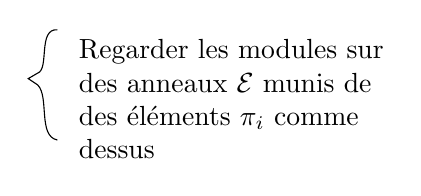
\begin{tikzpicture}[x=1cm,y=1cm]
\node[anchor=north west,align=left] at (.4,1.4) {Regarder les modules sur\\\deleted{des} anneaux $\mathcal E$ munis \deleted{de}\\des éléments $\pi_i$ comme\\dessus};
\draw (.25,1.4) .. controls (0,1.42) and (.15,.9) .. (0,.85) --(-.12,.78) --(0,.7) .. controls (.15,.55) and (0,.05) .. (.25,0);
\end{tikzpicture}}}

3. \deleted{Nous voulons} Partons enfin d'une \deleted{algèbre}\inserted{anneau} graduée $\mathcal E^*$ \deleted{sur $k$}, et posons nous la question de l'existence et \uline{l'unicité} d'une famille $(\pi_i)_{i\in\mathbb Z}$ d'éléments de $\mathcal E^*$, \inserted{satisfaisant $(1.1.)$} définissant la graduation, par $(1.3.)$ (donc par $(1.4)$). On \deleted{supp} suppose ici que
\mspage{3}

\scanpage{5}
\mspage{3}
\deleted{les $\pi_i$ \unsure{de} degré zéro}, et \deleted{que} l'on voudra que
\figure{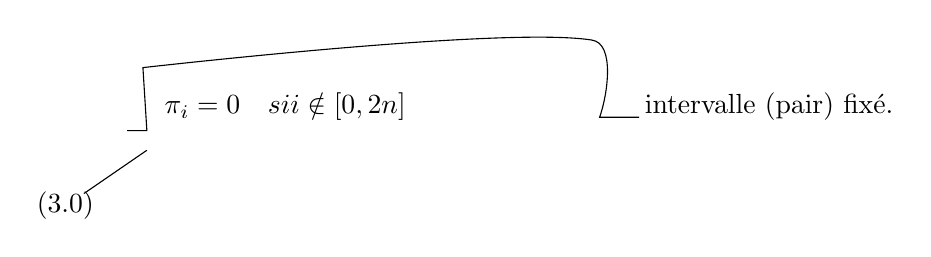
\begin{tikzpicture}[x=1cm,y=1cm]
\node[anchor=west] at (.8,.55) {$\pi_i=0\quad\text{si }i\notin[0,2n]$};
\node[anchor=west] at (6.9,.55) {intervalle \inserted{(pair)} fixé.};
\node[anchor=east] at (.15,-.7) {$(3.0)$};
\draw (.45,.25)--(.7,.25)--(.65,1.05) .. controls (2,1.2) and (5.4,1.55) .. (6.35,1.4) .. controls (6.65,1.36) and (6.55,.7) .. (6.45,.42)--(6.95,.42);
\draw (.7,0)--(-.1,-.55);
\end{tikzpicture}}
\deleted{Supp} On s'occupe ici de l'\uline{unicité}. \deleted{Supposons, établi l'unicité}

Notons d'abord que
\[
\mathcal E^0\ni u\quad\Longleftrightarrow\quad(u\pi_i=\pi_i u\quad\forall i)
\]
donc $\mathcal E^0$ est le commutant de la $k$-algèbre engendrée par les $\pi_i$. Donc les $\pi_i$ sont dans le centre $\mathfrak Z(\mathcal E^0)$ de $\mathcal E^0$, et ce sont des projecteurs \inserted{mutuellement} orthogonaux de somme $1$ de cet anneau commutatif. Supposons déterminés déjà les $\pi_\alpha$ pour $\alpha\notin[i,2n-i]$, \inserted{$i<n$,} et déterminons $\pi_i$ et $\pi_{2n-i}$ [i.e. $\pi_\alpha$ pour $\alpha\notin[i+1,2n-i-1]$.]
\inserted{\figure{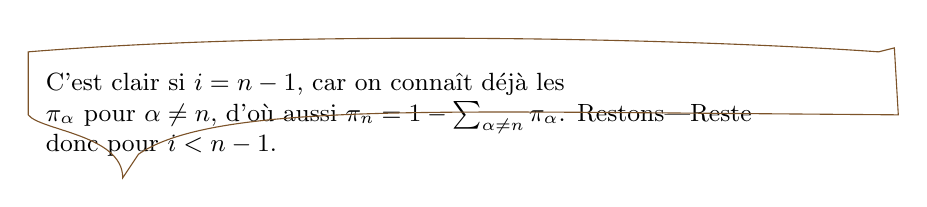
\begin{tikzpicture}[x=1cm,y=1cm]
\node[anchor=north west,align=left,font=\small] at (.2,.8) {C'est clair si $i=n-1$, car on connaît déjà les\\$\pi_\alpha$ pour $\alpha\neq n$, d'où aussi $\pi_n=1-\sum_{\alpha\neq n}\pi_\alpha$. \unsure{Restons|Reste}\\donc pour $i<n-1$.};
\draw[draw=brown!65!black] (.1,.95) .. controls (3.8,1.25) and (8.8,1.1) .. (10.9,.95) --(11.1,1.0)--(11.15,.15)--(7.5,.18) .. controls (4.5,.2) and (2.3,.2) .. (1.5,-.35) --(1.3,-.65) .. controls (1.3,-.1) and (.25,-.05) .. (.1,.15)--cycle;
\end{tikzpicture}}}
On connaît donc
\[
\varphi_i=\deleted{\unsure{1-\sum\pi_\alpha}}\left(1-\sum_{\alpha<i}\pi_i\right)=\sum_{\alpha\geq i}\pi_\alpha,
\quad\text{et}\quad
\psi_{2n-i}=\left(1-\sum_{\alpha>2n-i}\pi_i\right)=\sum_{\alpha\leq 2n-i}\pi_\alpha
\]
donc aussi la composante
\[
\unsure{ou|Or}\quad\psi_{2n-i}\deleted{\unsure{\varphi}}\mathcal E^{2n-2i}\varphi_i
=\sum_\alpha\psi_{2n-i}\pi_{\alpha+(2n-2i)}\mathcal E\pi_\alpha\varphi_i)
\]
Or
\[
\pi_\alpha\varphi_i=\begin{cases}0&\text{si }\alpha<i\\\pi_\alpha&\text{si }\alpha\geq i\end{cases}
\quad\text{et}\quad
\psi_{2n-i}\pi_{\alpha+(2n-2i)}=
\begin{cases}
0&\text{si }\inserted{\alpha+(2n-2i)>2n-i}\quad\text{i.e. }\alpha>i\\
\pi_{\alpha+(2n-2i)}&\text{si }\inserted{\alpha\leq i}
\end{cases}
\]
donc le terme d'indice $\alpha$ de la somme $\sum$ est nul sauf si $\alpha=i$, auquel cas il est égal à
\[
\pi_{i+(2n-2i)}\mathcal E\pi_i=\pi_{2n-i}\mathcal E\pi_i=\mathcal E_{2n-i,i}.
\]
Donc la connaissance des $\pi_\alpha$ pour $\alpha\notin[i,2n-i]$ implique la connaissance de $\mathcal E_{\deleted{\unsure{i,2n-i}}\inserted{2n-i,i}}$ \deleted{\unsure{Considéré|Considé}}

La condition qui va impliquer l'unicité \deleted{\illegible{1}} de $u_i$,
\mspage{4}

\scanpage{6}
\mspage{4}
$u_{2n-i}$ est donc la \deleted{qui} conjonction des suivantes :
\[
\begin{array}{l}(3.1.)_i\\[18pt](3.2)_i\end{array}
\quad\left.\begin{array}{l}\Bigl[
\bigl(u\in\mathfrak Z\mathcal E^0,\ \deleted{\unsure{\forall\alpha}\ \pi_\alpha u=0\ (\text{\unsure{pour}}\ \alpha\neq i),}\ 
\figure{\begin{tikzpicture}[baseline=(e.base)]\node[draw,ellipse,double,double distance=.6pt,inner sep=2pt] (e) {$\mathcal E_i^{2n-i}$};\end{tikzpicture}}u=0\bigr)
\Longrightarrow\deleted{u=0}\inserted{\pi_i u=0},\\[12pt]
\bigl(u\in\mathfrak Z\mathcal E^0,\ \deleted{\pi_\alpha u=0\ (\text{\unsure{pour}}\ \alpha\neq2n-i),}\ u\mathcal E_i^{2n-i}=0\bigr)
\Longrightarrow\deleted{u=0}\inserted{\pi_{2n-i}u=0}
\end{array}\right]
\]
En effet, la relation $(3.1.)$ implique que \deleted{$\pi_i(\mathfrak Z\mathcal E^0)$}\inserted{l'annulateur de $\pi_i$ dans $\mathfrak Z\mathcal E^0$} est l'idéal des $u\in\mathfrak Z\mathcal E^0$ tels que $\mathcal E_i^{2n-i}u=0$; or dans un anneau commutatif, un idempotent est connu quand on connaît son annulateur. De même pour $\pi_{2n-i}$, son annulateur dans $\mathfrak Z\mathcal E^0$ est formé des $u\in\mathfrak Z\mathcal E^0$ tels que $u\mathcal E_i^{2n-i}=0$.

En même temps, les conditions $(3.1.)_i$, $(3.2.)_i$ pour tt $i$, donnent un \deleted{condition} procédé pour déterminer de proche en proche les $\pi_i$.

\figure{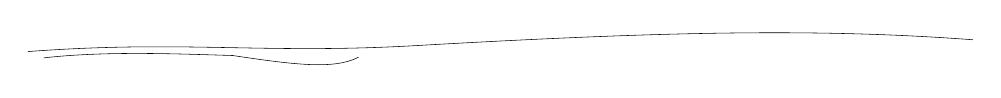
\begin{tikzpicture}[x=1cm,y=1cm]\draw[line width=.2pt] (0,0) .. controls (2,.15) and (3,-.04) .. (5,.08) .. controls (8,.25) and (10,.30) .. (12,.15);\draw[line width=.2pt] (.2,-.08) .. controls (1,.01) and (1.9,-.03) .. (2.6,-.05) .. controls (3.4,-.17) and (3.9,-.23) .. (4.2,-.07);\end{tikzpicture}}

4. Lorsque $\mathcal E^*$ est comme dans 1., une condition suffisante pour avoir $(3.1)_i$ \inserted{ou v. $(3.2)_i$} est la \deleted{suff} suivante

$(4.1)_i$ L'intersection des noyaux des $\unsure{v|u}:M^i\longrightarrow M^{2n-i}$, pour $v\in\mathcal E_i^{2n-i}$, est réduite à $0$.

$(4.2)_i$ La somme des images des $v:M^i\longrightarrowM^{2n-i}$, pour $v\in\mathcal E_i^{2n-i}$, est \deleted{\unsure{à}} égale à $M^{2n-i}$.

Ces deux conditions sont satisfaites si on a

$(4.3)_i$ Il existe \inserted{$v:M^i-M^{2n-i}$,} $v\in\mathcal E_i^{2n-i}$, qui est un isom. de
\mspage{5}

\scanpage{7}
\mspage{5}
façon équivalente, il existe un $v\in\mathcal E^{2n-2i}$, tel que le morphisme induit $v:M^i-M^{2n-i}$ soit un isomorphisme.

On peut transformer ceci de la façon suivante :
\[
\left\{\begin{aligned}
&\exists\ v_i\in\mathcal E^{2n-2i},\quad w_i\in\mathcal E^{-(2n-2i)},\quad\text{tels que l'on ait}\\
&(w_iv_i-1)\pi_i=0,\quad(v_iw_i-1)\pi_{2n-i}=0
\end{aligned}\right.
\tag*{$(4.4)_i$}
\]
Or, sans plus supposer que $\mathcal E^*$ se réalise à l'aide d'un $M^*$, on voit aussitôt que $(4.4)_i$ implique $(3.1)_i$ et $(3.2)_i$. En effet, quitte à remplacer $v,w$ par $v\pi_i=\pi_{2n-i}v$, $w\pi_{2n-i}=\pi_iw$, on peut supposer $v,w$ dans $\mathcal E_i^{2n-i}$, $\mathcal E_{2n-i}^i$. Si alors \deleted{\unsure{u}} $u\in\mathcal E^{(0)}$ est tel que $\mathcal E_i^{2n-i}u=0$, donc $vu=0$, on aura $wvu\pi_i\deleted{=0}=0$ i.e. $wv\pi_i u=0$ donc $\pi_i u=0$ (car $wv\pi_i=\pi_i$). De $=$ pour $(3.2)_i$, en utilisant la dernière relation $(4.4.)_i$.

\margin{\figure{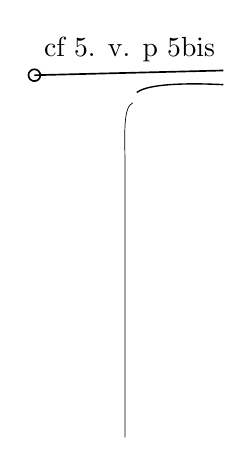
\begin{tikzpicture}[x=1cm,y=1cm]
\node[anchor=south west] at (0,4.65) {cf 5. v. p 5bis};
\draw[line width=.6pt] (0,4.6)--(2.4,4.66);
\draw[line width=.6pt] (0,4.6) circle (.075);
\draw[line width=.5pt] (1.3,4.38) .. controls (1.45,4.5) and (2.0,4.5) .. (2.4,4.48);
\draw[line width=.25pt] (1.25,4.25) .. controls (1.12,4.2) and (1.15,3.8) .. (1.15,3.5)--(1.15,0);
\end{tikzpicture}}}

6. Nous allons étudier de façon plus détaillée un cas où les conditions $(4.4)$ sont satisfaites. Pour ceci, partons encore du cas particulier $M^*$, \inserted{$\mathcal E^*$ sous-algèbre graduée de $\operatorname{End}(M^*)$,} et supposons qu'on ait un
\[
L\in\mathcal E^{(2)}
\tag{6.0}
\]
qui ait la propriété que
\mspage{6}

\scanpage{8}
\figure{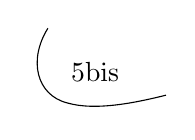
\begin{tikzpicture}[x=1cm,y=1cm]
\node at (.7,.45) {\mspage{5bis}};
\draw (.1,1.0) .. controls (-.15,.6) and (-.05,.15) .. (.35,.05) .. controls (.7,-.05) and (1.2,.05) .. (1.6,.15);
\end{tikzpicture}}
5. On peut aussi donner une condition d'\uline{existence} des $\pi_i$, liée aux conditions $(4.4)$. Pour ceci, on suppose que $\mathcal E$ est contenu dans un sur-anneau gradué $\mathcal F$ [p.ex. \inserted{l'anneau} des endom. d'un $M^*$ comme dans 1.] pour lequel les $\pi_i$ satisfont $(1.1.)$ et les relations correspondantes à $(1.3)$ (avec $\mathcal E$ remplacé par $\mathcal F$) sont satisfaites; \inserted{(et $(3.0)$: $\pi_i=0$ si $i\notin[0,2n]$)} Supposons que $\forall i$, la condition $(4.4)_i$ soit satisfaite, (avec $v_i,w_i\in\mathcal E$ bien sûr). On va en conclure que
\[
\pi_i\in\mathcal E\quad\text{pour tt }i.
\tag{5.1}
\]
\deleted{\unsure{Raisonnons par récurrence sur $i$.}}\inserted{Supposons prouvé \deleted{que} déjà $\pi_\alpha\in\mathcal E$ si $\alpha\notin[i,2n-i]$,} où $i<n$, et prouvons que l'on peut remplacer $i$ par $i+1$, \inserted{i.e. $\pi_i$ et $\pi_{2n-i}\in\mathcal E$.}\inserted{Trivial si $i=n-1$, supposons que $i\leq n-2$.}

Notons que, avec les notations de 3., \deleted{\unsure{on a}}\inserted{on a $\varphi_i,\psi_{2n-i}\in\mathcal E$, d'où} \deleted{\unsure{remplaçons} $v_i,\inserted{w_i}$ par} \deleted{\unsure{alors}}\inserted{donc} $\psi_{2n-i}v_i\varphi_i$, $\varphi_iw_i\psi_{2n-i}\in\mathcal E$, i.e.
\[
\left\{\begin{aligned}
\inserted{v'_i={}}\psi_{2n-i}v_i\varphi_i&=\pi_{2n-i}v_i\pi_i\in\mathcal E\\
\inserted{w'_i={}}\varphi_iw_i\psi_{2n-i}&=\pi_iw_i\pi_{2n-i}\in\mathcal E
\end{aligned}\right.
\]
et \uline{co}mme \deleted{donc}
\[
w'_iv'_i=\pi_iw_i\pi_{2n-i}v_i\pi_i
\inserted{\quad\text{car }w_i\pi_{2n-i}=\pi_iw_i}\]
\[
=\pi_i\pi_iw_iv_i\pi_i
\inserted{\quad\text{car }w_iv_i\pi_i=\pi_i}
=\pi_i^3=\pi_i.
\]
et de $=$ \deleted{$\unsure{=\pi_i}$} $v'_iw'_i=\pi_{2n-i}$, on conclut que $\pi_i\in\mathcal E$, $\pi_{2n-i}\in\mathcal E$.
\mspage{7}

\scanpage{9}
\mspage{6}
\[
L^{n-i}|M^i:\quad M^i\longrightarrow M^{2n-i}\quad\text{est un isom.}
\tag*{$(6.1)_i$}
\]
Ceci implique déjà $(4.1)_i$ et $(4.2)_i$ donc $(3.1)_i$ et $(3.2)_i$; \inserted{\figure{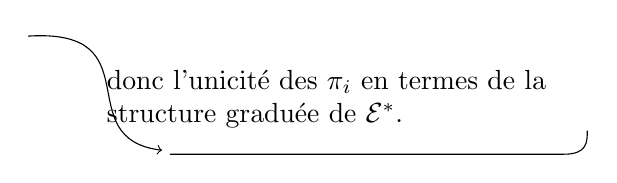
\begin{tikzpicture}[x=1cm,y=1cm]
\node[align=left,text width=6cm] at (1,0) {donc l'\uline{unicité} des $\pi_i$ en termes de la structure graduée de $\mathcal E^*$.};
\draw[->] (-3,.8) .. controls (-1.4,.9) and (-2.5,-.5) .. (-1.3,-.65);
\draw (-1.2,-.7) -- (3.8,-.7) .. controls (4.1,-.7) and (4.1,-.55) .. (4.1,-.4);
\end{tikzpicture}}} Supposons de plus

$(6.2)_i$ L'inverse de l'isom. $(6.1)$ est \deleted{\unsure{dans $\mathcal E_{2n-i}^i$}} induit par un élément de $\mathcal E^{-(2n-2i)}$.

\deleted{Ceci} L'ensemble des deux conditions $(6.1)$ et $(6.2)$, équivaut [en termes intrinsèques : $\mathcal E^*$, muni de $L\in\mathcal E^2$ si on suppose déjà les $\pi_i\in\mathcal E^*$]
\[
\left\{\begin{aligned}
&\exists\ w_i\in\mathcal E^{-(2n-2i)}\quad\text{tel qu'on ait}\\
&(w_iL^{n-i}-1)\pi_i=0,\quad(L^{n-i}w_i-1)\pi_{2n-i}=0
\end{aligned}\right.
\tag*{$(6.3.)_i$}
\]
Cette condition à son tour (indépendamment de la donnée préliminaire d'un $M^*$) implique $(4.4)_i$, \deleted{et on a donc $(3.1)_i$ et $(3.2)_i$}, \figure{\begin{tikzpicture}[x=1cm,y=1cm]
\node[align=center] at (0,.55) {\inserted{(en vertu des\\ n° 4, 5)}};
\node at (2.4,.65) {\inserted{$\pi_i\in\mathcal E$ et,}};
\node at (.65,-.1) {donc};
\draw (-1.2,.5) .. controls (-1.5,-.15) and (-.9,.1) .. (0,.1) .. controls (.8,.1) and (1.25,.2) .. (1.3,-.3);
\draw (1.4,.5) .. controls (2,.5) and (1.9,-.1) .. (2,-.35) .. controls (1.8,.35) and (3,.3) .. (3.6,.6);
\end{tikzpicture}} l'\uline{unicité} des $\pi_i$ en termes des conditions \figure{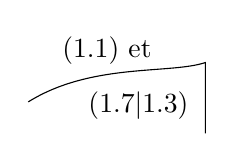
\begin{tikzpicture}[x=1cm,y=1cm]
\node at (0,.45) {$(1.1)$ et};
\node at (.4,-.25) {$(\unsure{1.7|1.3})$};
\draw (-1,-.2) .. controls (-.2,.3) and (.8,.15) .. (1.25,.3) -- (1.25,-.6);
\end{tikzpicture}}.

Revenons à $M^*$, et $L$ satisfaisant à $(6.1)_i$. Nous avons vu comment \deleted{la} cette condition implique la \uline{décomposition de} $M^*$ en termes \deleted{\unsure{can.}} de morceaux primitifs
\[
\left\{\begin{aligned}
M^i&\simeq P^i+LP^{i-2}+L^2P^{i-4}\quad\text{---}\\
M^{2n-i}&\simeq L^{n-i}P^i+L^{n-i+1}P^{i-2}\quad\text{---}
\end{aligned}\right.\qquad\bigg|\quad\text{si }i\leq n
\tag{6.4}
\]
On désigne par $\pi_{i,\alpha}$ la projection de $M^i$ sur $L^\alpha P^{i-2\alpha}$, par $\pi_{2n-i,\alpha}$ celle de $M^{2n-i}$ sur $L^{n-i+\alpha}P^{i-2\alpha}$,
\mspage{8}

\scanpage{10}
\mspage{7}
On a aussi l'hom. $\Lambda$ de degré $-2$, défini par
\[
\left\{\quad\cdot\ \cdot\ \cdot\ \cdot\ \cdot\ \cdot\right.
\tag{6.5}
\]
\uline{Théorème} Les conditions suivantes \inserted{(i) à (iii)} sont équivalentes

(i) Les conditions \inserted{$(6.1)_i$ et} $(6.2)_i$ pour tt $i$, et les $\pi_i\in\mathcal E$.

\deleted{\unsure{(ii)} [Une graduation de $\mathcal E^*$ peut être définie par des $\pi'_i$, et pour un \deleted{\illegible{2}} tel choix;]\par
\unsure{(ii)} \unsure{Les conditions} $(6.3)_i$ pour tt $i$ (avec $\pi_i$ \unsure{remplacé par} $\pi'_i$,....)}
\margin{\figure{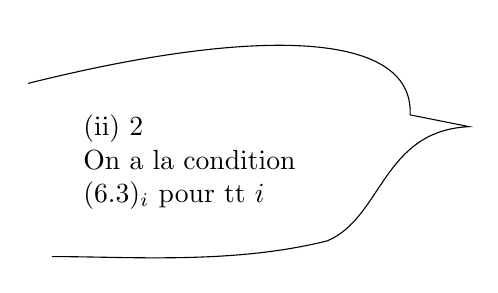
\begin{tikzpicture}[x=1cm,y=1cm]
\node[align=left,text width=4.2cm] at (0,0) {(ii) \deleted{\illegible{2}}\\On a la condition\\$(6.3)_i$ pour tt $i$};
\draw (-2.8,1) .. controls (0,1.7) and (2.1,1.7) .. (2.05,.6) -- (2.8,.45) .. controls (1.7,.4) and (1.7,-.7) .. (1,-1) .. controls (-.2,-1.3) and (-1.5,-1.2) .. (-2.5,-1.2);
\end{tikzpicture}}}

(iii) \deleted{L'hom.}\inserted{On a} \inserted{$(6.1)_i$ pour tt $i$, (\unsure{défin.|défini|définit|définissant} $\Lambda$) et}
\[
\uline{\Lambda\in\mathcal E^{(-2)}}
\tag{6.6}
\]
\deleted{\unsure{(iv)}} Ces conditions impliquent de plus

(iv) Les $\pi_{i,\alpha}$ sont dans $\mathcal E$, \deleted{les $\pi_i$ sont dans $\mathcal E$.}

(v) Les $\pi_i\in\mathcal E$, \inserted{et ils} sont \deleted{les seuls projecteurs}\inserted{définis comme formant \inserted{\figure{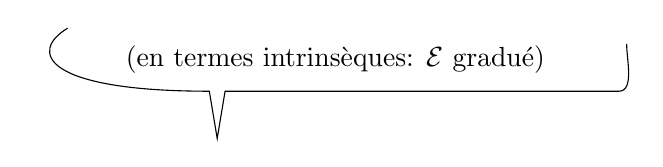
\begin{tikzpicture}[x=1cm,y=1cm]
\node at (0,.3) {(en termes intrinsèques: $\mathcal E$ gradué)};
\draw (-3.4,.7) .. controls (-3.9,.4) and (-3.7,-.1) .. (-1.6,-.1) -- (-1.5,-.7) -- (-1.4,-.1) -- (3.6,-.1) .. controls (3.8,-.1) and (3.7,.3) .. (3.7,.5);
\end{tikzpicture}}}} la seule famille d'éléments de $\mathcal E$ satisfaisant $(1.1.)$ et $(1.3)$ (a) ou b), au choix...., \unsure{$\mathcal E$|\deleted{$\mathcal E$}} ou encore $(1.4)$....).

\deleted{(vi) L'élément $\Lambda$ de $\mathcal E^{(-2)}$ est uniquement déterminé, \deleted{\unsure{par les}} (en termes de \inserted{l'anneau gradué} $\mathcal E^*$ et l'élt $L\in\mathcal E^{(1)}$, par les conditions suivantes :
\[
\left\{\begin{aligned}
L\Lambda&=1-\sum_{0\leq i\leq n}\pi_{i,0}\\
\Lambda L&=1-\sum_{n\leq i\leq2n}\pi_{i,0}
\end{aligned}\right.
\tag{6.7}
\]}

\uline{Dém.} L'équivalence de (i) et (ii) est claire, et le fait que i est impliqué par (iii) (en prenant $w_i=\Lambda^{\unsure{(}n-i\unsure{)}}$). \deleted{\unsure{Il}}\inserted{Reste à} prouver que (i), (ii) impliquent (iii) à (vi). On \deleted{sait déjà}\inserted{a déjà indiqué} que ça implique \deleted{$(6.7)$} (v).
\mspage{9}

\scanpage{11}
\mspage{8}
Prouvons (iv). Supposons prouvé
\[
\pi_{j\alpha}\in\mathcal E\quad\text{pour}\quad j\notin[i,2n-i]
\tag{6.7}
\]
où $i\leq n$, et prouvons que
\deleted{\[\pi_{j\alpha}\in\mathcal E\quad\text{pour}\quad j\in\]}
\[
\pi_{j\alpha}\in\mathcal E\quad\text{pour }j=i\text{ ou }j=2n-i,
\tag{6.7'}
\]
ce qui prouvera (iv) \inserted{\figure{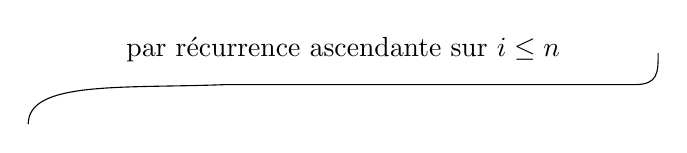
\begin{tikzpicture}[x=1cm,y=1cm]
\node at (0,.25) {par récurrence ascendante sur $i\leq n$};
\draw (-4,-.7) .. controls (-4,-.15) and (-2.8,-.25) .. (-1.5,-.2) -- (3.7,-.2) .. controls (4,-.2) and (4,-.05) .. (4,.2);
\end{tikzpicture}}}. Pour prouver $6.8.$ on procède par récurrence \deleted{\unsure{sur}} descendante sur $\alpha$, en supposant que.
\[
\deleted{\pi_{j\alpha}}\quad\pi_{i,\alpha'}\in\mathcal E,\quad\pi_{2n-i,\alpha'}\in\mathcal E\quad\text{si }\alpha'>\alpha,
\tag{6.8}
\]
et on en conclura que
\[
\pi_{i,\alpha}\in\mathcal E,\quad\pi_{2n-i,\alpha}\in\mathcal E.
\tag{6.8'}
\]
\deleted{Car \deleted{doit} prouvera bien $(6.7')$, puisque on peut démarrer la récurrence ($\pi_{i,\alpha}=\pi_{2n-i,\alpha}=0$ si $\alpha$ grand). Si $\alpha=0$, on gagne grâce à la relation
\[
\sum_\alpha\pi_{i,\alpha}=\pi_i\quad\text{donc}\quad\pi_{i,0}=\pi_i-\sum_{\alpha\geq1}\pi_{i\alpha},
\tag{6.9}
\]
donc il suffit d'envisager le cas $\alpha\geq1$.}

Posons
\[
q_{i,\alpha}=1-\sum_{\alpha'>\alpha}\pi_{i,\alpha'}=\sum_{\alpha'\leq\alpha}\pi_{i,\alpha}
\]
donc grâce à $(6.8)$ on a
\[
q_{i,\alpha}\in\mathcal E\quad\deleted{\unsure{\mathcal E}}
\]
\mspage{10}

\scanpage{12}
\mspage{9}
Alors on voit que
\[
L^{n-i+\alpha}q_{i\alpha}:M^i-M^{2n-i+2\alpha}
\]
est nul sur les $L^{\alpha'}P^{i-2\alpha'}$ pour $\alpha'\neq\alpha$, et que sur $L^\alpha P^{i-2\alpha}$, \deleted{il} son composé avec
\[
P^{i-2\alpha}\xrightarrow{L^\alpha}L^\alpha P^{i-2\alpha}
\]
n'est autre que l'isom
\[
L^{n-i-2\alpha}:P^{i-2\alpha}\RightarrowL^{n-i+2\alpha}P^{i-2\alpha}\subset M^{2n-i+2\alpha}.
\]
Il s'ensuit aussitôt que on a
\[
\pi_{i,\alpha}=L^\alpha w_{i-2\alpha}L^{n-i+\alpha}q_{i\alpha}=L^\alpha w_{i-2\alpha}L^{n-i+\alpha}(1-\sum_{\alpha'>\alpha}\pi_{i,\alpha'}
\tag{6.9}
\]
ce qui donne bien $\pi_{i\alpha}\in\mathcal E$. \deleted{Cela prouve (iv).}
Si $i<n$, il faut, égalt $\pi_{2n-i,\alpha}\in\mathcal E$. On
\deleted{Reste à prouver \inserted{(iii)} $\Lambda\in\mathcal E$. Il suffit de \deleted{\unsure{prendre}.} poser
\[
q_{2n-i,\alpha}=1-\sum_{\alpha'>\alpha}\pi_{2n-i,\alpha'}
\]
et on voit alors que
\[
\deleted{\unsure{L^{n-i+\alpha}}}L^\alpha q_{2n-i,\alpha}:M^{2n-i}-M^{2n-i+2\alpha}
\]}
le déduit p. ex. de la formule
\[
\pi_{2n-i,\alpha}=L^{n-i}\pi_{i,\alpha}w_i\deleted{\unsure{\pi_{2n-i}}}
\tag{6.10}
\]
Cela prouve \inserted{\figure{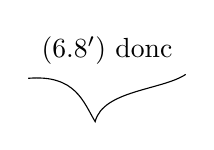
\begin{tikzpicture}[x=1cm,y=1cm]
\node at (0,.25) {$(6.8')$ donc};
\draw (-1,-.1) .. controls (-.4,-.05) and (-.3,-.4) .. (-.15,-.65) .. controls (-.05,-.25) and (.7,-.25) .. (1,-.05);
\end{tikzpicture}}} (iv). Reste : prouver (iii) $\Lambda\in\mathcal E$.

Comme on a
\[
\Lambda=\sum_{j,\alpha\,\deleted{\unsure{j\leq n}}}\deleted{\unsure{\Lambda}}\Lambda\pi_{j,\alpha}\quad\deleted{\unsure{+\sum_{\alpha\neq0}\Lambda}\quad\unsure{+\sum_{0\leq i\leq n}\pi_{i,0}\Lambda}}
\tag{6.11}
\]
il suffit de prouver que $\Lambda\pi_{i\alpha}\deleted{\Lambda\pi_{i,\alpha}}\in\mathcal E$.
\mspage{11}

\scanpage{13}
\mspage{10}
Or si $i\leq n$, on aura
\[
\left\{\quad\Lambda\pi_{i0}=0,\qquad\Lambda\pi_{i\alpha}=L^{\alpha-1}w_{i-2\alpha}L^{n-i+\alpha}\pi_{i\alpha}\quad\text{si }\alpha\geq1,\right.
\tag{6.12}
\]
\deleted{et si $j>n$, on aura
\[
\Lambda\pi_{j\alpha}=L
\tag{6.12}
\]}
\[
\Lambda\pi_{2n-i,\alpha}=L^{n-i+\alpha-1}w_{i-2\alpha}\deleted{\unsure{\pi_{2n-i,\alpha}}}L^\alpha\pi_{2n-i,\alpha}\quad(\text{si }i\leq n-1)
\tag{6.13}
\]
\margin{Les conditions envisagées impliquent évidemment (iv) : prouver que (iv) implique (ii). Il suffit de prouver en fait que l'on a alors $\pi_i=\pi'_i$. \uline{Démonstration à fournir.}}

\uline{Remarque} Voici un système de conditions déterminant de façon unique les éléments $\Lambda\in\mathcal E^{(2)},\ \pi_{i,\alpha}\in\mathcal E^{(0)}$ en termes de $L$, et des $\pi_i\deleted{\unsure{\alpha}}$ (dont nous avons déjà une caractérisation intrinsèque par ailleurs, en termes de l'anneau gradué $\mathcal E$) :
\margin{\deleted{$\unsure{\pi_{2n-i}}$}}
\[
\left\{\begin{aligned}
\textcircled{1}\quad &(\Lambda^{n-i}L^{n-i}-1)\pi_i=0
\qquad\textcircled{2}\quad\deleted{\pi_{2n-i}}(L^{n-i}\Lambda^{n-i}-1)\deleted{\pi_{2n-i}}\pi_{2n-i}=0\\
\textcircled{3}\quad &\pi_{i,\alpha}=L^\alpha\deleted{\unsure{w_{i-2\alpha}}}\inserted{\Lambda^{n-i+2\alpha}}L^{n-i+\alpha}\bigl(1-\sum_{\alpha'>\alpha}\pi_{i,\alpha'}\bigr)\\
\textcircled{4}\quad &\pi_{2n-i,\alpha}=L^{n-i}\pi_{i,\alpha}\Lambda^{n-i}\\
&\deleted{\Lambda=\sum_{j,\alpha}\Lambda\pi_{j\alpha}}\\
\textcircled{5}\quad &\Lambda\pi_{i,0}=0\qquad\deleted{\unsure{\alpha}}\\
\textcircled{6}\quad &\Lambda\pi_{i\alpha}=L^{\alpha-1}\Lambda^{n-i+2\alpha}L^{n-i+\alpha}\pi_{i\alpha}\quad\text{si }\alpha\geq1\\
\textcircled{7}\quad &\Lambda\pi_{2n-i,\alpha}=L^{n-i+\alpha-1}\Lambda^{n-i+2\alpha}L^\alpha\pi_{2n-i,\alpha}\quad\text{si }\alpha\leq n-1\\
\textcircled{8}\quad &\Lambda=\sum_{j,\alpha}\Lambda\pi_{j\alpha}
\end{aligned}\right.
\tag{6.14}
\]
(dans ttes ces formules, on suppose $i\leq n$).

Dans ces huit formules, on peut d'ailleurs remplacer les quatre dernières par les suivantes \inserted{\figure{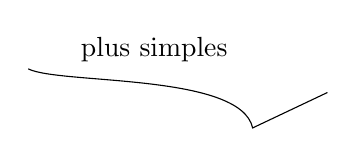
\begin{tikzpicture}[x=1cm,y=1cm]
\node at (0,.35) {plus simples};
\draw (-1.6,.1) .. controls (-1.2,-.1) and (1.1,.05) .. (1.25,-.65) -- (2.2,-.2);
\end{tikzpicture}}} :
\mspage{12}

\scanpage{14}
\figure{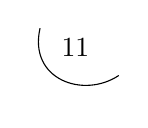
\begin{tikzpicture}[x=1cm,y=1cm]
\node at (0,0) {\mspage{11}};
\draw (-.45,.25) .. controls (-.6,-.4) and (.1,-.65) .. (.55,-.35);
\end{tikzpicture}}
\[
\left\{\begin{aligned}
L\Lambda&=1-\sum_{0\leq i\leq n}\pi_{i,0}\\
\Lambda L&=1-\sum_{n\leq j\leq2n}\pi_{\deleted{2}j,0}
\end{aligned}\right.
\tag{6.15}
\]
\deleted{Quant aux $\pi_{j,0}$, ils sont déterminés par les}

\uline{Question} Donner un système de \deleted{\unsure{générateurs}} relations entre les $\Lambda,L$ exclusivement, \deleted{\unsure{et}} de relations exprimant les $\pi_i$ comme polynômes en $L,\Lambda$ .... --- qui définissent $\Lambda$ en termes de $L$ et des $\pi_i$ ....
\margin{\figure{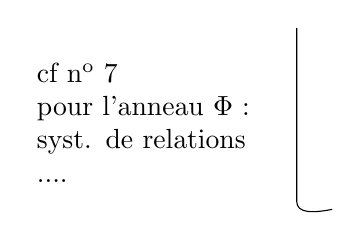
\begin{tikzpicture}[x=1cm,y=1cm]
\node[align=left,text width=3cm] at (0,0) {cf n\textsuperscript{o} 7\\pour l'anneau $\Phi$ :\\syst. de relations ....};
\draw (1.8,1.2) -- (1.8,-1) .. controls (1.8,-1.15) and (2,-1.15) .. (2.25,-1.1);
\end{tikzpicture}}}

7. Revenant à un anneau gradué abstrait $\mathcal E$, muni d'un
\[
L\in\mathcal E^{(2)},
\]
on veut abstraire la situation qui précède, sans utiliser $M^*$, en termes des propriétés du seul anneau \deleted{$\mathcal E$} gradué $\mathcal E^*$ muni de $L\in\mathcal E^{(2)}$.
Partons pour ceci \deleted{de} d'un module libre $\mathbf M_0$ de rang $2n$ sur $\mathbb Z$, muni d'une $2$-forme alternée non dégénérée \inserted{\figure{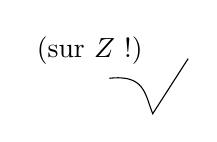
\begin{tikzpicture}[x=1cm,y=1cm]
\node at (0,.25) {(sur $\mathbb Z$ !)};
\draw (.25,-.1) .. controls (.7,-.05) and (.7,-.3) .. (.8,-.55) -- (1.25,.15);
\end{tikzpicture}}} $\xi_0\in\bigwedge^2\mathbf M_0$, \inserted{\figure{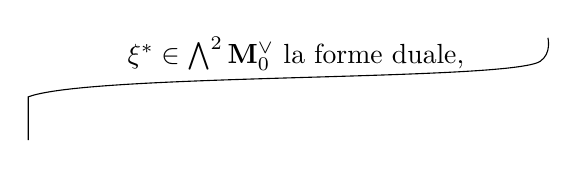
\begin{tikzpicture}[x=1cm,y=1cm]
\node at (0,.3) {$\xi^*\in\bigwedge^2\mathbf M_0^\vee$ la forme duale,};
\draw (-3.4,-.8) -- (-3.4,-.25) .. controls (-2.6,.05) and (2.7,-.05) .. (3.1,.2) .. controls (3.25,.3) and (3.2,.5) .. (3.2,.5);
\end{tikzpicture}}} soit \deleted{$\xi$} $\mathbf M_0^*=\bigwedge\mathbf M_0$, et considérons sur $\mathbf M_0^*$ les opérateurs
\[
\mathbf Lx=\xi_0x,\qquad\boldsymbol\Lambda_0x=\xi_0^*\mathbin{\lrcorner}x
\]
et considérons l'algèbre
\[
\Phi_0=\mathbb Z[\mathbf L_0,\boldsymbol\Lambda_0]\subset\operatorname{End}_{\mathbb Z}(\mathbf M_0^*)
\]
\margin{anneau gradué.}
Notons que $\operatorname{End}(\mathbf M_0^*)$, \inserted{\figure{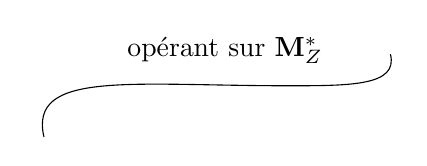
\begin{tikzpicture}[x=1cm,y=1cm]
\node at (0,.35) {opérant sur $\mathbf M_{\mathbb Z}^*$};
\draw (-2.3,-.75) .. controls (-2.5,.1) and (-1.2,-.1) .. (.8,-.1) .. controls (1.6,-.1) and (2.2,-.1) .. (2.1,.3);
\end{tikzpicture}}} muni de $\unsure{\mathbf L|\mathbf L_0}$, satisfait à la condition de $(6.1)\unsure{(\omega)|(i)|_i}$, \deleted{\unsure{donc}} et \deleted{$\xi$} $\boldsymbol\Lambda_0$ est l'opérateur associé défini par $(6.5)$.
\mspage{13}
